% Provenance (never printed): cycle 3 "La planete Terre" (natural phenomena
% and the risks they bring: storms, floods, droughts, earthquakes, eruptions;
% warnings and the right behaviour); see sources/book1/PROVENANCE.md.
% Book 1, grade 5, chapter 3.
\chapter{Natural Hazards}\label{ch:g5:natural-hazards}

It is Friday evening. On the radio, the music stops and a calm voice reads
a warning: a strong \omterm{def:g5:natural-hazards:storm}{storm} will reach the \omterm{def:g1:landscapes-around-us:water}{coast} tonight, with very strong
winds and heavy \omterm{def:g4:clouds-rain-snow:precipitation}{rain}. People are asked to stay indoors from nine o'clock
and to tie down or bring in anything the wind could carry away.

Lena's family gets to work. Her father brings the garden chairs and the
table into the shed. Her mother checks that the torches work and puts
spare batteries on the kitchen table. Lena fills two big bottles with
water. By nine o'clock, everyone is inside, and the wind is already
howling.

\begin{omfigure}
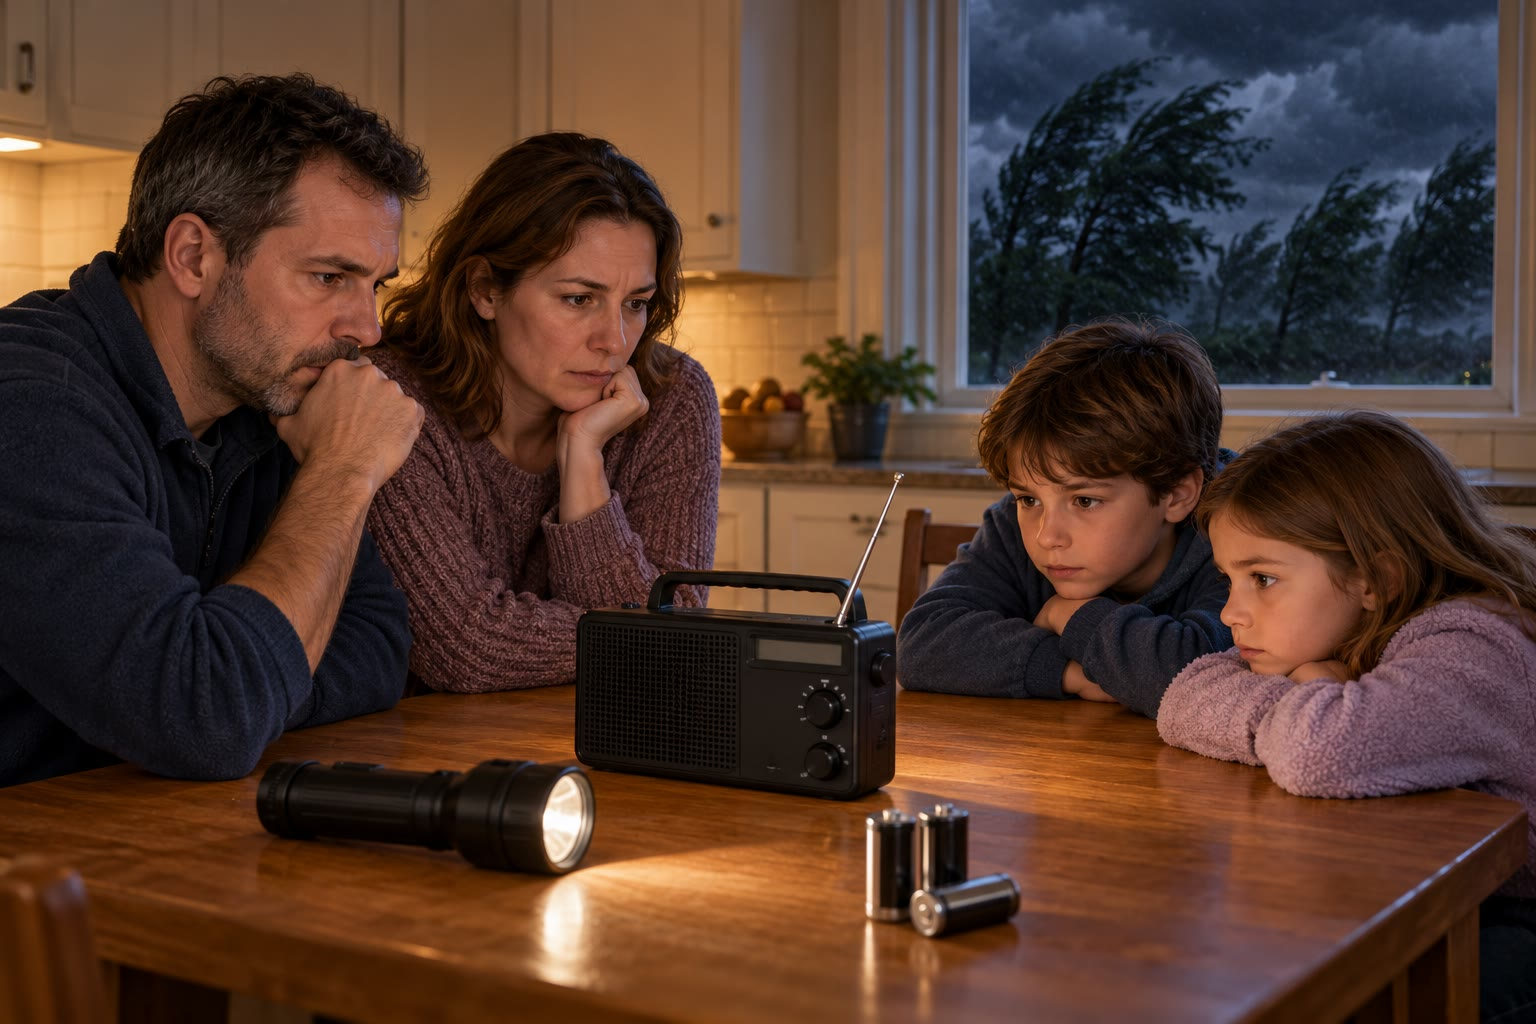
\includegraphics[width=0.5\linewidth]{images/book1/ai/g5-radio-warning.jpg}

{\small A family listens to a \omterm{def:g5:natural-hazards:storm}{storm} warning on the radio, with torches and
spare batteries ready.}
\end{omfigure}

\begin{recall}
A \omterm{def:g4:volcanoes-earthquakes-first-look:volcano}{volcano} can erupt, throwing out \omterm{def:g4:volcanoes-earthquakes-first-look:eruption}{lava}, ash and gas; an \omterm{def:g4:volcanoes-earthquakes-first-look:earthquake}{earthquake} is a
sudden shaking of the ground; in an \omterm{def:g4:volcanoes-earthquakes-first-look:earthquake}{earthquake}, we drop, cover and hold on
(\cref{ch:g4:volcanoes-earthquakes-first-look}). A \omterm{def:g1:landscapes-around-us:water}{river} that receives more
water than its channel can hold \omterm{def:g5:water-shapes-the-land:flood}{floods} its \omterm{def:g5:water-shapes-the-land:flood}{floodplain}
(\cref{ch:g5:water-shapes-the-land}). Each place has its own \omterm{def:g5:weather-and-climate:climate}{climate}, and
the hot, temperate and cold zones go round the \omterm{def:g3:continents-and-oceans:globe}{globe}
(\cref{ch:g5:weather-and-climate}).
\end{recall}

\section{What a natural hazard is}

Nature is not always calm. The wind can blow strongly enough to break
trees, \omterm{def:g1:landscapes-around-us:water}{rivers} can \omterm{def:g5:water-shapes-the-land:flood}{flood}, the ground can shake. These events are part of
how the Earth works: they happened long before there were people, and
they will go on happening.

\begin{definition}[Natural hazard]\label{def:g5:natural-hazards:hazard}
A \emph{natural hazard}\index{natural hazard} is a natural event that can
harm people or damage what they have built: a \omterm{def:g5:natural-hazards:storm}{storm}, a \omterm{def:g5:water-shapes-the-land:flood}{flood}, a \omterm{def:g5:natural-hazards:drought}{drought}, an
\omterm{def:g4:volcanoes-earthquakes-first-look:earthquake}{earthquake}, a volcanic \omterm{def:g4:volcanoes-earthquakes-first-look:eruption}{eruption}, a \omterm{def:g5:natural-hazards:landslide}{landslide}{\ldots}
\end{definition}

We can sort \omterm{def:g5:natural-hazards:hazard}{natural hazards} by where they come from: from the air, from
water, or from the ground.

\begin{omfigure}
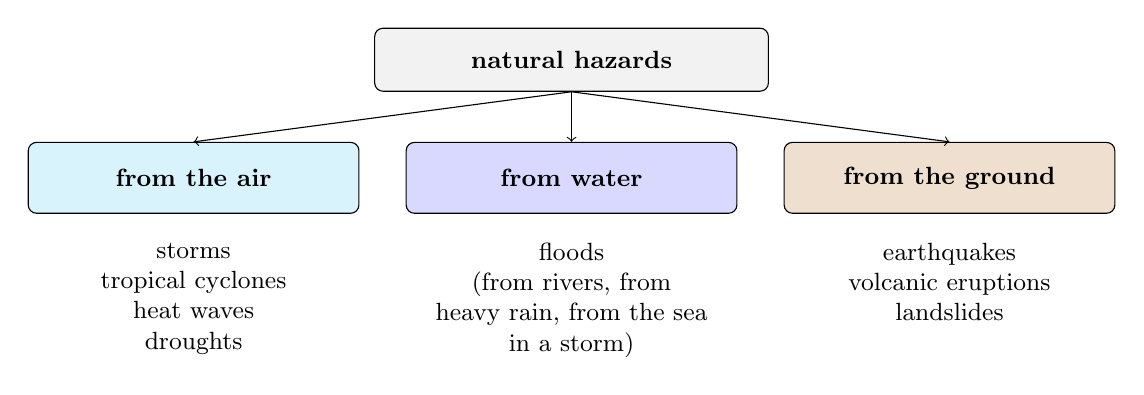
\begin{tikzpicture}[font=\small, box/.style={draw, rounded corners=3pt,
    minimum width=4.2cm, minimum height=0.9cm, align=center}]
  \node[box, fill=cyan!15, font=\small\bfseries] (A) at (0,0) {from the air};
  \node[box, fill=blue!15, font=\small\bfseries] (W) at (4.8,0) {from water};
  \node[box, fill=brown!25, font=\small\bfseries] (G) at (9.6,0) {from the ground};
  \node[align=center, anchor=north] at (0,-0.7) {storms\\tropical cyclones\\heat waves\\droughts};
  \node[align=center, anchor=north] at (4.8,-0.7) {floods\\(from rivers, from\\heavy rain, from the sea\\in a storm)};
  \node[align=center, anchor=north] at (9.6,-0.7) {earthquakes\\volcanic eruptions\\landslides};
  \node[draw, rounded corners=3pt, fill=gray!10, font=\small\bfseries,
    minimum width=5cm, minimum height=0.8cm] (N) at (4.8,1.5) {natural hazards};
  \draw[->] (N.south) -- (A.north);
  \draw[->] (N.south) -- (W.north);
  \draw[->] (N.south) -- (G.north);
\end{tikzpicture}

{\small The \omterm{def:g5:natural-hazards:hazard}{natural hazards}, sorted by where they come from.}
\end{omfigure}

\section{Hazards from the air}

\begin{definition}[Storm]\label{def:g5:natural-hazards:storm}
A \emph{storm}\index{storm} is a time of very strong wind, usually with
heavy \omterm{def:g4:clouds-rain-snow:precipitation}{rain} or \omterm{def:g4:clouds-rain-snow:precipitation}{snow}, and sometimes with thunder and lightning.
\end{definition}

A strong \omterm{def:g5:natural-hazards:storm}{storm} breaks branches, knocks down trees, tears tiles off roofs,
and can throw garden chairs through windows. On the \omterm{def:g1:landscapes-around-us:water}{coast}, its wind piles
the \omterm{def:g2:water-on-earth:ocean}{sea} up against the shore and sends huge waves over the \omterm{def:g2:water-on-earth:ocean}{sea} walls.

The most powerful \omterm{def:g5:natural-hazards:storm}{storms} on Earth form over warm tropical \omterm{def:g2:water-on-earth:ocean}{seas}. They are
huge, spinning \omterm{def:g5:natural-hazards:storm}{storms}: from space, they look like a giant spiral of
\omterm{def:g4:clouds-rain-snow:cloud}{clouds}, with a calm, clear hole in the middle, the eye. Around the eye
blow the strongest winds. The same kind of \omterm{def:g5:natural-hazards:storm}{storm} has different names in
different \omterm{def:g2:water-on-earth:ocean}{oceans}: it is called a \emph{hurricane} in the North Atlantic and
in the eastern Pacific, a \emph{typhoon} in the north-west Pacific, and a
\emph{tropical cyclone} in the South Pacific and the Indian \omterm{def:g2:water-on-earth:ocean}{Ocean}.
% ledger: noaa:cyclone-names

\begin{omfigure}
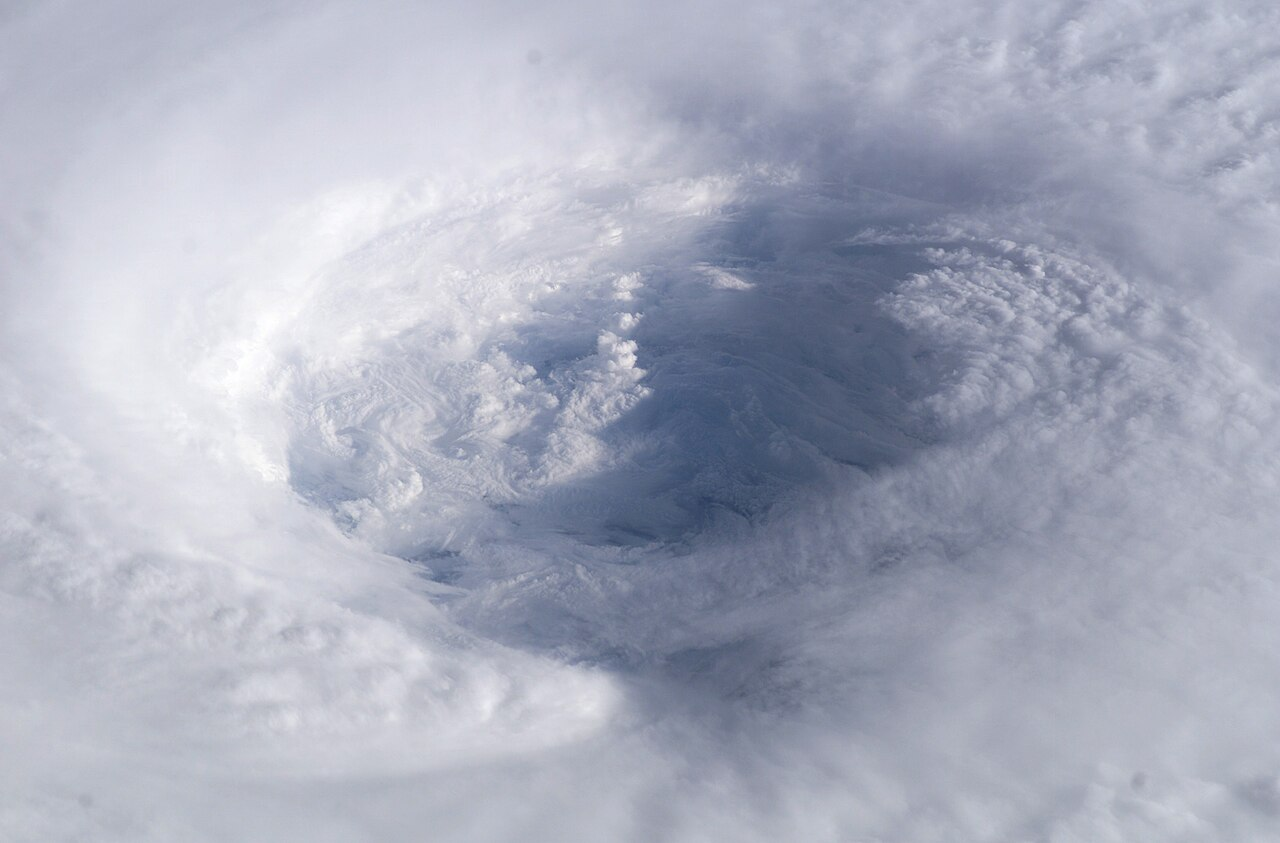
\includegraphics[width=0.5\linewidth]{images/book1/g5-hurricane-isabel-iss.jpg}

{\small Looking down into the eye of Hurricane Isabel, over the Atlantic
\omterm{def:g2:water-on-earth:ocean}{Ocean} in September 2003, from the International Space Station: a wall of
\omterm{def:g4:clouds-rain-snow:cloud}{cloud} around a calmer centre. Photograph: NASA (public domain).}
% ledger: nasa:isabel-iss
\end{omfigure}

Some hazards from the air are slow and quiet. A \emph{heat wave} is a
period of several days and nights that are much hotter than usual. It is
dangerous above all for very old people, babies and the sick.

\begin{definition}[Drought]\label{def:g5:natural-hazards:drought}
A \emph{drought}\index{drought} is a long period, of months or even years,
with much less \omterm{def:g4:clouds-rain-snow:precipitation}{rain} than usual for that place. The soil dries out, \omterm{def:g1:landscapes-around-us:water}{rivers}
and \omterm{def:g1:landscapes-around-us:water}{lakes} shrink, crops wilt and die.
\end{definition}

A \omterm{def:g5:natural-hazards:drought}{drought} creeps up slowly: no one can say on which day it starts. But a
long \omterm{def:g5:natural-hazards:drought}{drought} can leave farmers without a harvest and towns short of water.

\begin{omfigure}
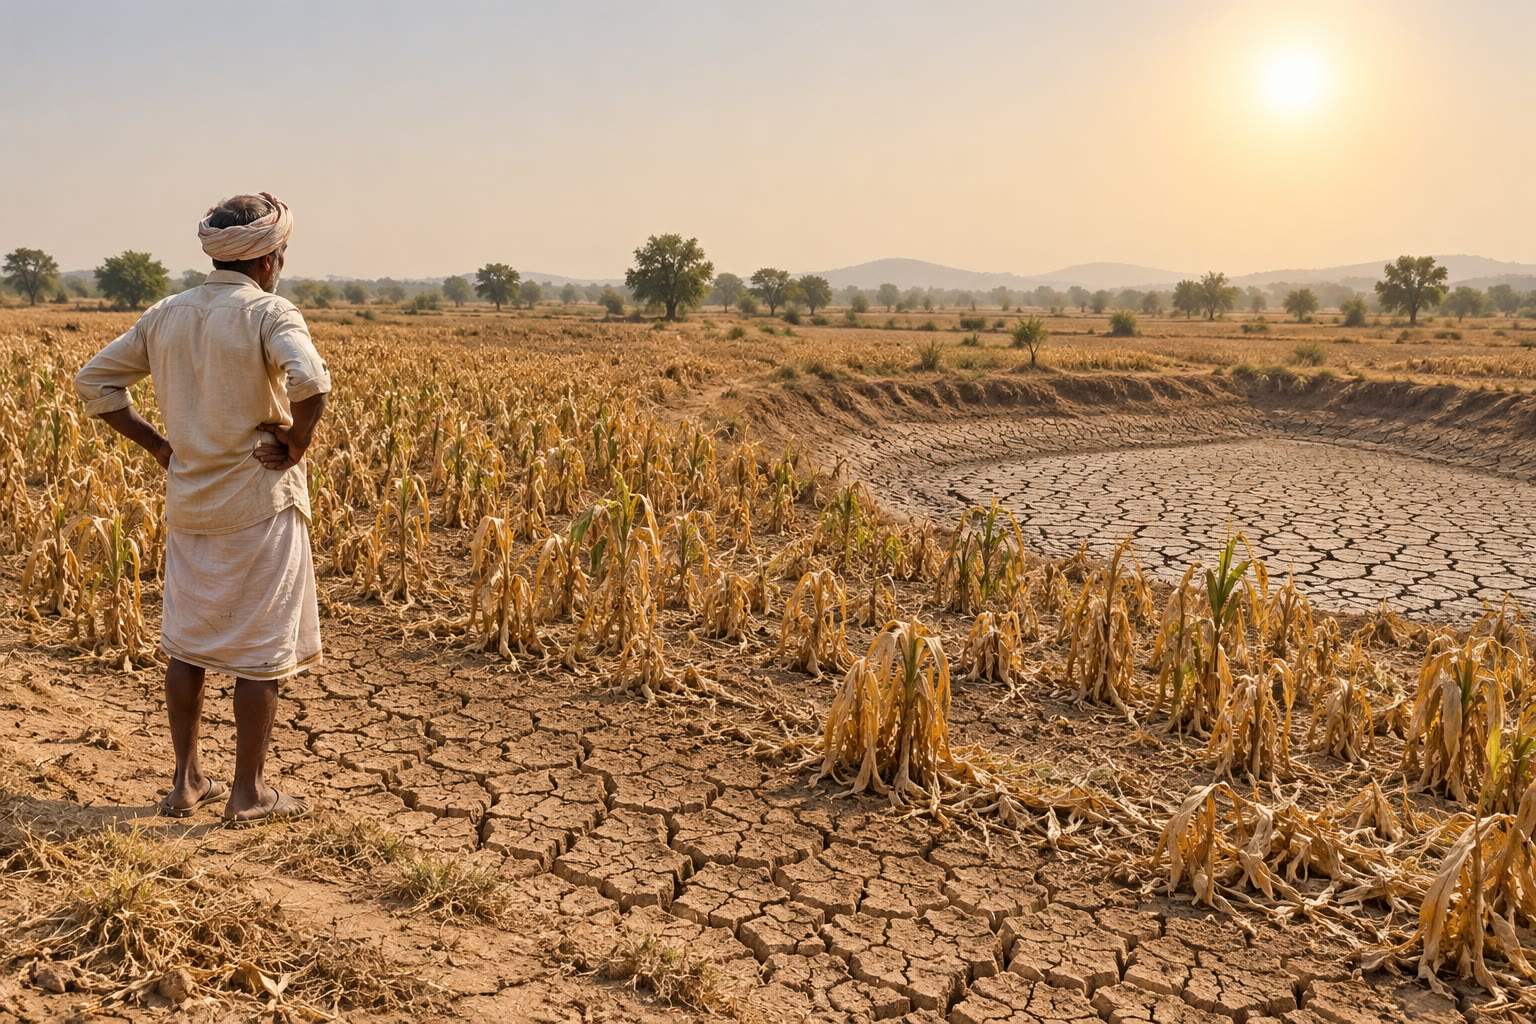
\includegraphics[width=0.42\linewidth]{images/book1/ai/g5-drought-field.jpg}

{\small A field in a long \omterm{def:g5:natural-hazards:drought}{drought}: the earth is cracked, the crops are
yellow and the pond has dried up.}
\end{omfigure}

\section{Hazards from water}

You already know the \omterm{def:g5:water-shapes-the-land:flood}{floods} of \omterm{def:g1:landscapes-around-us:water}{rivers} (\cref{ch:g5:water-shapes-the-land}).
After days of \omterm{def:g4:clouds-rain-snow:precipitation}{rain}, or when the \omterm{def:g4:clouds-rain-snow:precipitation}{snow} melts fast, a \omterm{def:g1:landscapes-around-us:water}{river} rises above its
banks and covers its \omterm{def:g5:water-shapes-the-land:flood}{floodplain}. Some \omterm{def:g5:water-shapes-the-land:flood}{floods} come very fast: a violent
downpour on a steep \omterm{def:g1:landscapes-around-us:landform}{valley} can turn a quiet stream into a roaring torrent
within an hour. Others come from the \omterm{def:g2:water-on-earth:ocean}{sea}, when a \omterm{def:g5:natural-hazards:storm}{storm} pushes the water up
onto a low \omterm{def:g1:landscapes-around-us:water}{coast}.

\section{Hazards from the ground}

You already know \omterm{def:g4:volcanoes-earthquakes-first-look:earthquake}{earthquakes} and volcanic \omterm{def:g4:volcanoes-earthquakes-first-look:eruption}{eruptions}
(\cref{ch:g4:volcanoes-earthquakes-first-look}). There is a third hazard
from the ground, and water often triggers it.

\begin{definition}[Landslide]\label{def:g5:natural-hazards:landslide}
A \emph{landslide}\index{landslide} is a mass of \omterm{def:g3:stones-pebbles-sand:rock}{rock}, earth or \omterm{def:g3:stones-pebbles-sand:sand}{mud} that
suddenly slides or falls down a slope.
\end{definition}

A steep slope soaked by long \omterm{def:g4:clouds-rain-snow:precipitation}{rains} becomes heavy and slippery, and it can
let go all at once. An \omterm{def:g4:volcanoes-earthquakes-first-look:earthquake}{earthquake} can also shake a slope loose. A \omterm{def:g5:natural-hazards:landslide}{landslide}
can bury a road, block a \omterm{def:g1:landscapes-around-us:water}{river}, or carry houses away.

\begin{omfigure}
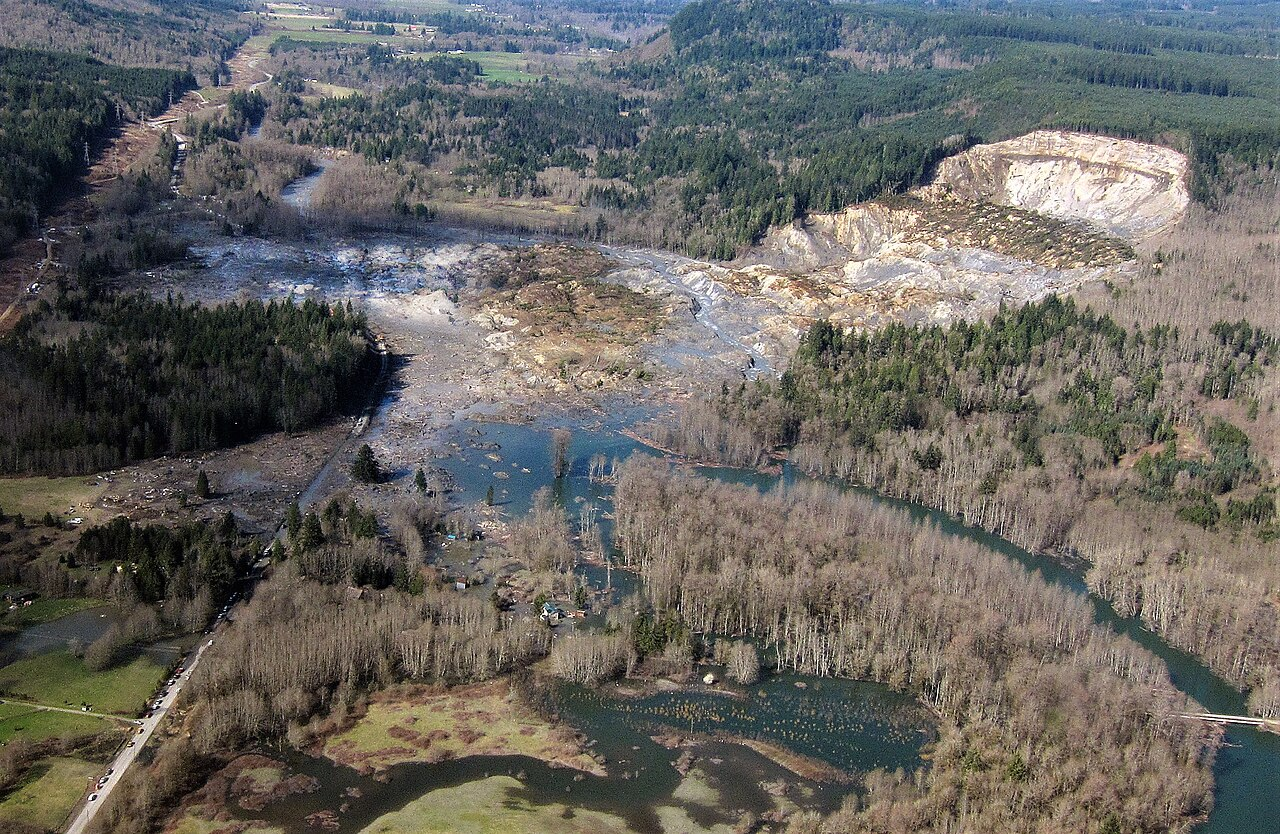
\includegraphics[width=0.6\linewidth]{images/book1/g5-landslide-washington.jpg}

{\small A large \omterm{def:g5:natural-hazards:landslide}{landslide} in Washington State, in the United States, in
2014, seen from an aircraft. The hillside on the right has collapsed; its
\omterm{def:g3:stones-pebbles-sand:sand}{mud} has spread across the whole \omterm{def:g1:landscapes-around-us:landform}{valley}, covered a road and blocked the
\omterm{def:g1:landscapes-around-us:water}{river}, which has flooded the woods upstream. Photograph: Mark Reid, U.S.
Geological Survey (public domain).}\label{fig:g5:natural-hazards:landslide}
% ledger: usgs:oso-aerial
\end{omfigure}

\section{From a hazard to a disaster}

A \omterm{def:g5:natural-hazards:storm}{storm} over the open \omterm{def:g2:water-on-earth:ocean}{ocean}, an \omterm{def:g4:volcanoes-earthquakes-first-look:earthquake}{earthquake} in an empty \omterm{def:g5:weather-and-climate:desert}{desert}, a \omterm{def:g5:water-shapes-the-land:flood}{flood} in
a \omterm{def:g1:landscapes-around-us:landform}{valley} where no one lives: these are \omterm{def:g5:natural-hazards:hazard}{natural hazards}, but they harm no
one. The same events become dangerous when they strike where people live.

\begin{definition}[Natural disaster]\label{def:g5:natural-hazards:disaster}
A \emph{natural disaster}\index{natural disaster} happens when a \omterm{def:g5:natural-hazards:hazard}{natural
hazard} strikes a place where people live and does great harm: people are
hurt or killed, homes are destroyed, roads, water and electricity are cut.
\end{definition}

\begin{omfigure}
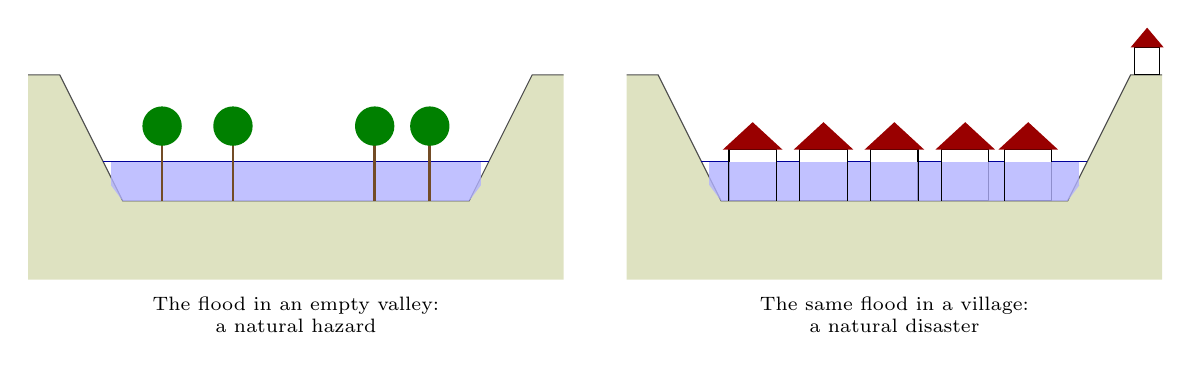
\begin{tikzpicture}[x=1cm, y=1cm, font=\scriptsize]
  \foreach \dx/\title in {0/{The flood in an empty valley:\\a natural hazard},
                          7.6/{The same flood in a village:\\a natural disaster}} {
    \begin{scope}[xshift=\dx cm]
      % valley sides
      \fill[green!25!brown!30] (0,0) -- (0,2.6) -- (0.4,2.6) -- (1.2,1.0) -- (5.6,1.0)
        -- (6.4,2.6) -- (6.8,2.6) -- (6.8,0) -- cycle;
      \draw[gray!60!black] (0,2.6) -- (0.4,2.6) -- (1.2,1.0) -- (5.6,1.0) -- (6.4,2.6) -- (6.8,2.6);
      % flood water over the whole valley floor
      \fill[blue!30, opacity=0.8] (1.05,1.2) -- (5.75,1.2) -- (5.6,1.0) -- (1.2,1.0) -- cycle;
      \fill[blue!30, opacity=0.8] (1.05,1.2) rectangle (5.75,1.5);
      \draw[blue!60!black] (0.95,1.5) -- (5.85,1.5);
      \node[align=center, anchor=north] at (3.4,-0.1) {\title};
    \end{scope}
  }
  % trees in the empty valley
  \foreach \x in {1.7,2.6,4.4,5.1} {
    \draw[brown!60!black, line width=1pt] (\x,1.0) -- (\x,1.75);
    \fill[green!50!black] (\x,1.95) circle (0.25);
  }
  % houses in the village valley
  \begin{scope}[xshift=7.6cm]
    \foreach \x in {1.6,2.5,3.4,4.3,5.1} {
      \fill[white, draw=black] (\x-0.3,1.0) rectangle (\x+0.3,1.65);
      \fill[red!60!black] (\x-0.38,1.65) -- (\x,2.0) -- (\x+0.38,1.65) -- cycle;
      \fill[blue!30, opacity=0.8] (\x-0.3,1.0) rectangle (\x+0.3,1.5);
    }
    % one house on the high ground, dry
    \fill[white, draw=black] (6.45,2.6) rectangle (6.77,2.95);
    \fill[red!60!black] (6.40,2.95) -- (6.61,3.2) -- (6.82,2.95) -- cycle;
  \end{scope}
\end{tikzpicture}

{\small The same \omterm{def:g5:water-shapes-the-land:flood}{flood} twice. In the empty \omterm{def:g1:landscapes-around-us:landform}{valley} it harms no one; where a
village has been built on the \omterm{def:g5:water-shapes-the-land:flood}{floodplain}, it fills the houses. The house
on the high ground stays dry.}
\end{omfigure}

We cannot stop a \omterm{def:g5:natural-hazards:storm}{storm} or an \omterm{def:g4:volcanoes-earthquakes-first-look:earthquake}{earthquake}. But we can do a great deal to
keep a hazard from becoming a disaster: build away from \omterm{def:g5:water-shapes-the-land:flood}{floodplains} and
from the foot of unstable slopes, make buildings strong, watch the \omterm{def:g1:watching-the-weather:weather}{weather}
and the ground, warn people in time, and teach everyone what to do.

\subsection*{Warnings}

\omterm{def:g1:watching-the-weather:weather}{Weather} services watch the sky day and night. When a \omterm{def:g5:natural-hazards:storm}{storm}, a heat wave or
a \omterm{def:g5:water-shapes-the-land:flood}{flood} is coming, they send out warnings by radio, television, phone and
the internet. Many countries use colours, from the calmest to the most
serious.

\begin{omfigure}
\begin{tikzpicture}[font=\small, wstep/.style={draw=black!60, minimum width=2.6cm,
    minimum height=0.8cm, font=\small\bfseries, rounded corners=2pt}]
  \node[wstep, fill=green!45] (g) at (0,0) {green};
  \node[wstep, fill=yellow!60] (y) at (0.6,0.95) {yellow};
  \node[wstep, fill=orange!70] (o) at (1.2,1.9) {orange};
  \node[wstep, fill=red!65, text=white] (r) at (1.8,2.85) {red};
  \node[anchor=west] at ($(g.east)+(0.3,0)$) {no particular danger};
  \node[anchor=west] at ($(y.east)+(0.3,0)$) {be careful, keep informed};
  \node[anchor=west] at ($(o.east)+(0.3,0)$) {be prepared: danger is likely};
  \node[anchor=west] at ($(r.east)+(0.3,0)$) {great danger: act now, follow the instructions};
\end{tikzpicture}

{\small A ladder of warning colours. The exact meanings differ from one
country to another: always listen to the instructions given with the
warning.}
\end{omfigure}

\begin{safety}
\textbf{In a \omterm{def:g5:natural-hazards:storm}{storm}.} Stay indoors, away from windows. Do not go out to
look, and keep away from trees, which can fall, and from fallen electric
wires.

\textbf{In a \omterm{def:g5:water-shapes-the-land:flood}{flood}.} Move to higher ground or to an upper floor. Never
walk, cycle or ride in a car through \omterm{def:g5:water-shapes-the-land:flood}{flood} water: a little fast water is
enough to knock you over or carry a car away.

\textbf{In a heat wave.} Drink water often, stay in the shade or in a cool
room during the hottest hours, and check on elderly neighbours.

\textbf{In an \omterm{def:g4:volcanoes-earthquakes-first-look:earthquake}{earthquake}.} Drop, cover, hold on
(\cref{ch:g4:volcanoes-earthquakes-first-look}).

\textbf{Always.} Listen to the warnings and do what the people in charge
say, at once.
\end{safety}

\section{Exercises}

\begin{exercise}[$\star$]\label{exo:g5:natural-hazards:1}
\omterm{def:g5:natural-hazards:hazard}{Natural hazard} only, or \omterm{def:g5:natural-hazards:disaster}{natural disaster}?
\begin{enumerate}
  \item[(a)] An \omterm{def:g4:volcanoes-earthquakes-first-look:earthquake}{earthquake} shakes an empty \omterm{def:g5:weather-and-climate:desert}{desert}.
  \item[(b)] A \omterm{def:g5:natural-hazards:storm}{storm} tears the roofs off many houses in a town.
  \item[(c)] A \omterm{def:g5:natural-hazards:landslide}{landslide} falls into a \omterm{def:g1:landscapes-around-us:landform}{mountain} \omterm{def:g1:landscapes-around-us:landform}{valley} where no one lives.
  \item[(d)] A \omterm{def:g1:landscapes-around-us:water}{river} \omterm{def:g5:water-shapes-the-land:flood}{floods} a village and fills its houses with water.
\end{enumerate}
\end{exercise}

\begin{exercise}[$\star$]\label{exo:g5:natural-hazards:2}
Sort these hazards into three families (from the air, from water, from the
ground): a \omterm{def:g5:natural-hazards:landslide}{landslide}; a heat wave; a \omterm{def:g5:water-shapes-the-land:flood}{flood}; a volcanic \omterm{def:g4:volcanoes-earthquakes-first-look:eruption}{eruption}; a \omterm{def:g5:natural-hazards:storm}{storm}; a
\omterm{def:g5:natural-hazards:drought}{drought}; an \omterm{def:g4:volcanoes-earthquakes-first-look:earthquake}{earthquake}.
\end{exercise}

\begin{exercise}[$\star$]\label{exo:g5:natural-hazards:3}
What is a \omterm{def:g5:natural-hazards:drought}{drought}? Give two ways in which a long \omterm{def:g5:natural-hazards:drought}{drought} harms people.
\end{exercise}

\begin{exercise}[$\star$]\label{exo:g5:natural-hazards:4}
The radio announces a red \omterm{def:g5:natural-hazards:storm}{storm} warning for tonight. Give three things your
family should do.
\end{exercise}

\begin{exercise}[$\star$]\label{exo:g5:natural-hazards:5}
A great spinning \omterm{def:g5:natural-hazards:storm}{storm} with an eye forms over a warm tropical \omterm{def:g2:water-on-earth:ocean}{sea}. What is
it called if it strikes (a) the \omterm{def:g1:landscapes-around-us:water}{coast} of Florida, in the North Atlantic;
(b) Japan, in the north-west Pacific; (c) the \omterm{def:g1:landscapes-around-us:water}{coast} of India, on the Indian
\omterm{def:g2:water-on-earth:ocean}{Ocean}?
\end{exercise}

\begin{exercise}[$\star$]\label{exo:g5:natural-hazards:6}
Put the four warning colours in order, from the calmest to the most
serious. What should you do at the most serious level?
\end{exercise}

\begin{exercise}[$\star\star$]\label{exo:g5:natural-hazards:7}
Look at the photograph of the \omterm{def:g5:natural-hazards:landslide}{landslide} on
page~\pageref{fig:g5:natural-hazards:landslide}. Describe what the
\omterm{def:g5:natural-hazards:landslide}{landslide} did to the \omterm{def:g1:landscapes-around-us:landform}{valley}: to the hillside, to the road and to the \omterm{def:g1:landscapes-around-us:water}{river}.
Why is the land upstream now under water?
\end{exercise}

\begin{exercise}[$\star\star$]\label{exo:g5:natural-hazards:8}
Tom says: ``\omterm{def:g5:water-shapes-the-land:flood}{Floods} are natural, so nothing can be done about them.'' Lena
says: ``We cannot stop a \omterm{def:g1:landscapes-around-us:water}{river} from flooding, but we can stop a \omterm{def:g5:water-shapes-the-land:flood}{flood} from
becoming a disaster.'' Who is right? Explain with two examples.
\end{exercise}

\begin{exercise}[$\star\star$]\label{exo:g5:natural-hazards:9}
In an imaginary farming region, about 60 millimetres of \omterm{def:g4:clouds-rain-snow:precipitation}{rain} usually fall
each month. During a \omterm{def:g5:natural-hazards:drought}{drought}, only a quarter of the usual \omterm{def:g4:clouds-rain-snow:precipitation}{rain} fell in each
of four months.
\begin{enumerate}
  \item[(a)] How much \omterm{def:g4:clouds-rain-snow:precipitation}{rain} usually falls in four months?
  \item[(b)] How much fell during the \omterm{def:g5:natural-hazards:drought}{drought}, in the four months?
  \item[(c)] How much \omterm{def:g4:clouds-rain-snow:precipitation}{rain} was missing?
\end{enumerate}
\end{exercise}

\begin{exercise}[$\star\star$]\label{exo:g5:natural-hazards:10}
An imaginary town has 1\,200 homes. A quarter of them stand on the
\omterm{def:g5:water-shapes-the-land:flood}{floodplain} of its \omterm{def:g1:landscapes-around-us:water}{river}.
\begin{enumerate}
  \item[(a)] How many homes stand on the \omterm{def:g5:water-shapes-the-land:flood}{floodplain}?
  \item[(b)] The town helps the owners of a third of those homes to move to
        higher ground. How many homes are still on the \omterm{def:g5:water-shapes-the-land:flood}{floodplain}?
\end{enumerate}
\end{exercise}

\begin{exercise}[$\star\star\star$]\label{exo:g5:natural-hazards:11}
Two villages, far apart, are hit by \omterm{def:g5:natural-hazards:storm}{storms} of the same strength on the same
night. In the first, no one is hurt and the damage is small. In the second,
many houses are destroyed. Give at least three different reasons that could
explain the difference.
\end{exercise}
